 \documentclass[10pt, letterpaper]{article}
\usepackage[top=80pt,bottom=80pt,left=60pt,right=60pt]{geometry}
\usepackage{tabularx}
\usepackage{float}
\usepackage{amsmath} % for boxing equations
\usepackage{titling}
\newcommand{\subtitle}[1]{
  \posttitle{
    \par\end{center}
    \begin{center}\large#1\end{center}
    \vskip0.5em}
}
\usepackage{tikz}
\usepackage[section]{placeins}
\usepackage[utf8]{inputenc}
\usepackage{csvsimple}
\usepackage{subfig}

\begin{document}

  \title{Internal Assessment: The Impact of the Sphere's Radius on the Sphere's Angular Velocity}
  \subtitle {IB Physics II Period 6, Dr. Petach}
  \date{19 October 2015}
  \author{Jackson Chen}
  \maketitle

  \section{Exploration}

    \subsection{Research}

    The aim of the experiment is to investigate the relationship between radius and
    angular velocity for the linear motion of a sphere unraveling from a string at a
    fixed height. This will be done by changing the radius of the sphere that is being
    dropped through the use of various sizes balls that are unraveled from the string
    and then measuring the linear velocity of the falling ball using a photogate.
    The purpose of the string is to cause the ball to rotate while falling, due to the
    nature of its unraveling motion.

    Prior to the experiment, I derived a relationship between the radius and the angular
    velocity of the rotational motion of the falling ball by using the law of conservation of
    energy. Section \ref{sssec:derivation} will more specifically detail the derivation.
    The derived relationship predicted that radius and angular velocity will follow an inverse relationship.
    The experiment itself was to test whether Newtonian physics upheld this inverse
    relationship with tangible experimentation.

    \subsection{Personal Engagement}

    I have always been a fan of yo-yo's. One day while playing with a yo-yo, I noticed how
    quickly the yo-yo was spinning, which was made especially conspicuous by the bright design
    on the side of the yo-yo. I became curious, did the size of the yo-yo affect how quickly
    it spun? I took a smaller yo-yo and noticed that it seemed to spin more quickly.
    However, this was just a casual observation, not performed under standard experimentation
    conditions. Interested in seeing if this was truly the case, I came up with my research
    question: does the radius of a sphere affect its angular velocity?

    \subsection{Variables}
    The independent variable is the radius of the sphere. The dependent variable is the
    angular velocity of the ball as it passes through the photogate. The controlled variables
    include the height of the initial position of the ball that is attached to the clamp,
    material of the string, the photogate, and the properties of the surrounding environment.

    \subsection{Apparatus}
    \begin{itemize}
      \item Photogate
      \item Four different sizes balls that are relatively uniform spheres
      \item String
      \item DataWorks software that reads data from the photogate
      \item Ring stand with clamp
      \item Meter stick
    \end{itemize}

    \subsection{Procedure}
    \begin{enumerate}
      \item Attach a clamp to a ringstand
      \item Place a photogate toward the bottom of the ringstand so that the ball will drop through it.
      \item Connect the photogate to the DataWorks software, such that it reads the linear velocity of the falling ball
      \item Measure the height difference between the placement of the clamp and the photogate along the ring stand using a meter stick
      \item Pick a ball, measure it radius using a meter stick
      \item Tie one end of the string to a clamp attached to a ring stand, and the other end around the ball
      \item Carefully wrap the string around the ball until the ball is level with the clamp
      \item Drop the ball so that it falls through the photogate
      \item Record the linear velocity that is measured by the photogate
      \item Repeat steps 6 to 9 for six trials
      \item Repeat steps 5 through 10 for the four different balls
    \end{enumerate}

    \subsection{Experiment Setup}
    \begin{figure}[!htb]
      \centering
      \parbox{2.75in} {
        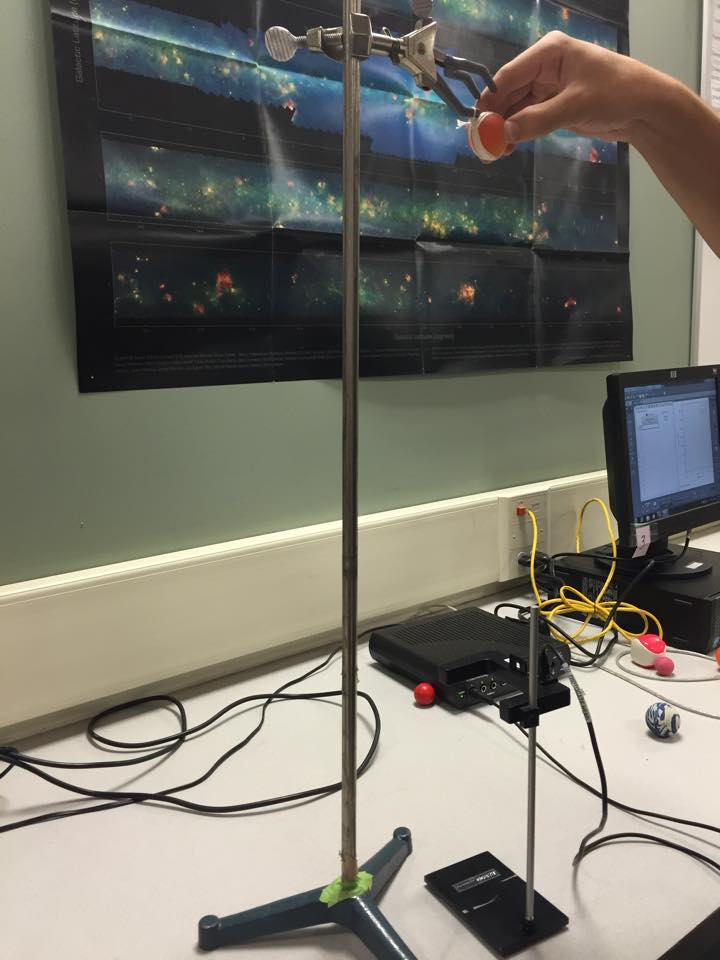
\includegraphics[scale=0.233]{img/setup.jpg}
        \caption{Picture of the experiment setup}
      }
      \begin{minipage}{2.75in}
        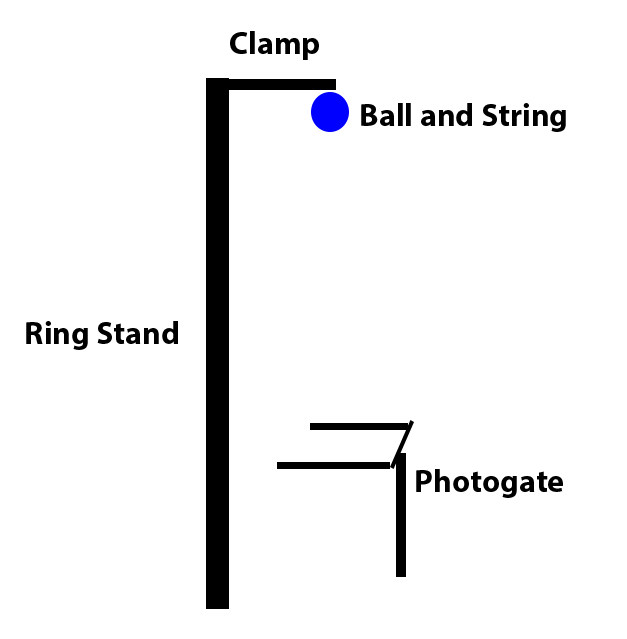
\includegraphics[scale=0.7]{img/apparatus.png}
        \caption{Diagram of the experiment setup}
      \end{minipage}
    \end{figure}

    \subsection{Data Collection}
      \begin{table}[H]
      \centering
      \begin{tabularx}{\linewidth}{>{\centering\arraybackslash}X>{\centering\arraybackslash}X>{\centering\arraybackslash}X }
        \hline \textbf{Trial} & \textbf{Radius (cm)} & \textbf{Linear Velocity (m/s)} \\ \hline
                1             & $2.34 \pm 0.05$      &  1.86 \\ \hline
                2             & $2.34 \pm 0.05$      &  1.81 \\ \hline
                3             & $2.34 \pm 0.05$      &  3.10 \\ \hline
                4             & $2.34 \pm 0.05$      &  2.50 \\ \hline
                5             & $2.34 \pm 0.05$      &  2.87 \\ \hline
                6             & $2.34 \pm 0.05$      &  2.20 \\ \hline
      \end{tabularx}
      \caption{Data for six trials with ball radius of 2.34 cm and height of $50.00 \pm 0.05$ cm.}
      \end{table}

      \begin{table}[H]
      \centering
      \begin{tabularx}{\linewidth}{>{\centering\arraybackslash}X>{\centering\arraybackslash}X>{\centering\arraybackslash}X }
        \hline \textbf{Trial} & \textbf{Radius (cm)} & \textbf{Linear Velocity (m/s)} \\ \hline
                1             &	$1.90 \pm 0.05$      & 2.12 \\ \hline
                2             &	$1.90 \pm 0.05$      & 2.38 \\ \hline
                3             &	$1.90 \pm 0.05$      & 2.98 \\ \hline
                4             &	$1.90 \pm 0.05$      & 2.23 \\ \hline
                5             &	$1.90 \pm 0.05$      & 2.35 \\ \hline
                6             &	$1.90 \pm 0.05$      & 2.23 \\ \hline
      \end{tabularx}
      \caption{Data for six trials with ball radius of 1.90 cm and height of $50.00 \pm 0.05$ cm.}
      \end{table}

      \begin{table}[H]
      \centering
      \begin{tabularx}{\linewidth}{>{\centering\arraybackslash}X>{\centering\arraybackslash}X>{\centering\arraybackslash}X }
        \hline \textbf{Trial} & \textbf{Radius (cm)} & \textbf{Linear Velocity (m/s)} \\ \hline
                1             &	$1.69 \pm 0.05$      &	3.32 \\ \hline
                2             &	$1.69 \pm 0.05$      &	3.18 \\ \hline
                3             &	$1.69 \pm 0.05$      &	2.22 \\ \hline
                4             &	$1.69 \pm 0.05$      &	3.91 \\ \hline
                5             &	$1.69 \pm 0.05$      &	2.85 \\ \hline
                6             &	$1.69 \pm 0.05$      &	3.63 \\ \hline
      \end{tabularx}
      \caption{Data for six trials with ball radius of 1.69 cm and height of $50.00 \pm 0.05$ cm.}
      \end{table}

      \begin{table}[H]
      \centering
      \begin{tabularx}{\linewidth}{>{\centering\arraybackslash}X>{\centering\arraybackslash}X>{\centering\arraybackslash}X }
        \hline \textbf{Trial} & \textbf{Radius (cm)} & \textbf{Linear Velocity (m/s)} \\ \hline
               1              &	$1.40 \pm 0.05$      &	2.91 \\ \hline
               2              &	$1.40 \pm 0.05$      &	3.62 \\ \hline
               3              &	$1.40 \pm 0.05$      &	3.62 \\ \hline
               4              &	$1.40 \pm 0.05$      &	2.31 \\ \hline
               5              &	$1.40 \pm 0.05$      &	3.67 \\ \hline
               6              &	$1.40 \pm 0.05$      &	3.41 \\ \hline
      \end{tabularx}
      \caption{Data for six trials with ball radius of 1.40 cm and height of $50.00 \pm 0.05$ cm.}
      \end{table}
  \section{Analysis}

    \subsection{Deriving the relationship between radius and angular velocity} \label{sssec:derivation}
      A relationship can be found between radius and angular velocity by using the law of conservation of energy.
      Effects of thermal energy (friction) from the string are negligible.
      \[ GPE = KE_{T} + KE_{R}\]
      \[ mgh = \frac{1}{2}mv^2 + \frac{1}{2}I \omega ^2 \]
      \[ mgh = \frac{1}{2}m(R \omega )^2 + \frac{1}{2} \left( \frac{2}{5}mR^2 \right) \omega ^2 \]
      \[ mgh = \frac{1}{2}mR^{2} \omega ^2 + \frac{1}{5}mR^{2} \omega ^2 \]
      The masses can be eliminated:
      \[ gh = \frac{7}{10}R^2 \omega ^2 \]
      \[ \omega ^2 = \frac{10gh}{7R^2} \]
      \[ \omega = \sqrt{\frac{10gh}{7R^2}} \]
      \begin{equation}
      \[ \omega = \boxed{ \frac{1}{R} \cdot \sqrt{\frac{10gh}{7}} } \]
      \end{equation}

    \subsection{Calculating angular velocity}
      Using Equation 1, derived above, the angular velocity can be calculated for each ball size.
      For radius 2.34 cm:
      \[ \omega = \frac{1}{0.234} \]

    \subsection{Averaging the six trials for each ball size and finding uncertainty}
      A sample calculation will be done for the set of data around the ball with radius 2.34 cm. \\\\
      Uncertainty for linear velocity can be calculated by dividing the linear velocity range by 2:
      \[ \frac{3.10 - 1.81}{2} = 0.65  \]
      Now to find the average:
      \[ \frac{1.86 + 1.81 + 3.10 + 2.50 + 2.87 + 2.20}{6} = 2.39 \frac{m}{s} \]

      \begin{table}[H]
      \centering
      \begin{tabularx}{\linewidth}{>{\centering\arraybackslash}X>{\centering\arraybackslash}X>{\centering\arraybackslash}X }
        \hline \textbf{Radius (cm)} & \textbf{Linear Velocity (m/s)} \\ \hline
                $2.34 \pm 0.05$     &	 $2.39 \pm 0.65$ \\ \hline
      \end{tabularx}
      \caption{Data for six trials with ball radius of 1.40 cm and height of $50.00 \pm 0.05$ cm.}
      \end{table}

    \subsection{Analyzing experiment evidence for radius vs angular velocity}

  \section{Evaluation}

\end{document}
